% =====================================================================
% Slide 9: Stage 3-4 -- DFT references -> MEAM single-element init
% (Stage 4's alpha table dropped: its a0/Ecoh duplicate the table below)
% =====================================================================
\begin{frame}{Stage 3--4: DFT References $\to$ MEAM Initialisation}
\begin{columns}[T]
\column{0.45\textwidth}
\centering
\scriptsize
\setlength{\tabcolsep}{4pt}
\renewcommand{\arraystretch}{0.95}
\begin{tabular}{llrrr}
\toprule
Element & Lat. & $a_{0}$ (\AA) & $E_{\mathrm{coh}}$ & $B$ (GPa) \\
\midrule
Al & FCC     & 4.047 & 3.611 &  77.5 \\
Cu & FCC     & 3.639 & 3.857 & 138.5 \\
Si & DIAMOND & 5.471 & 5.130 &  89.3 \\
Ti & HCP     & 2.915 & 6.284 & 114.5 \\
Zn & HCP     & 2.766 & 0.964 &  68.4 \\
Cr & BCC     & 2.848 & 3.964 & 213.1 \\
Fe & BCC     & 2.806 & 6.834 & 420.5 \\
Mg & HCP     & 3.177 & 1.483 &  47.8 \\
Mn & BCC     & 2.803 & 3.728 & 225.7 \\
Mo & BCC     & 3.169 &10.353 & 280.8 \\
\bottomrule
\end{tabular}\\[0.2em]
\textit{Elemental references}
($E_{\mathrm{coh}}$ in eV/atom; Birch--Murnaghan fits).

\column{0.54\textwidth}
\centering
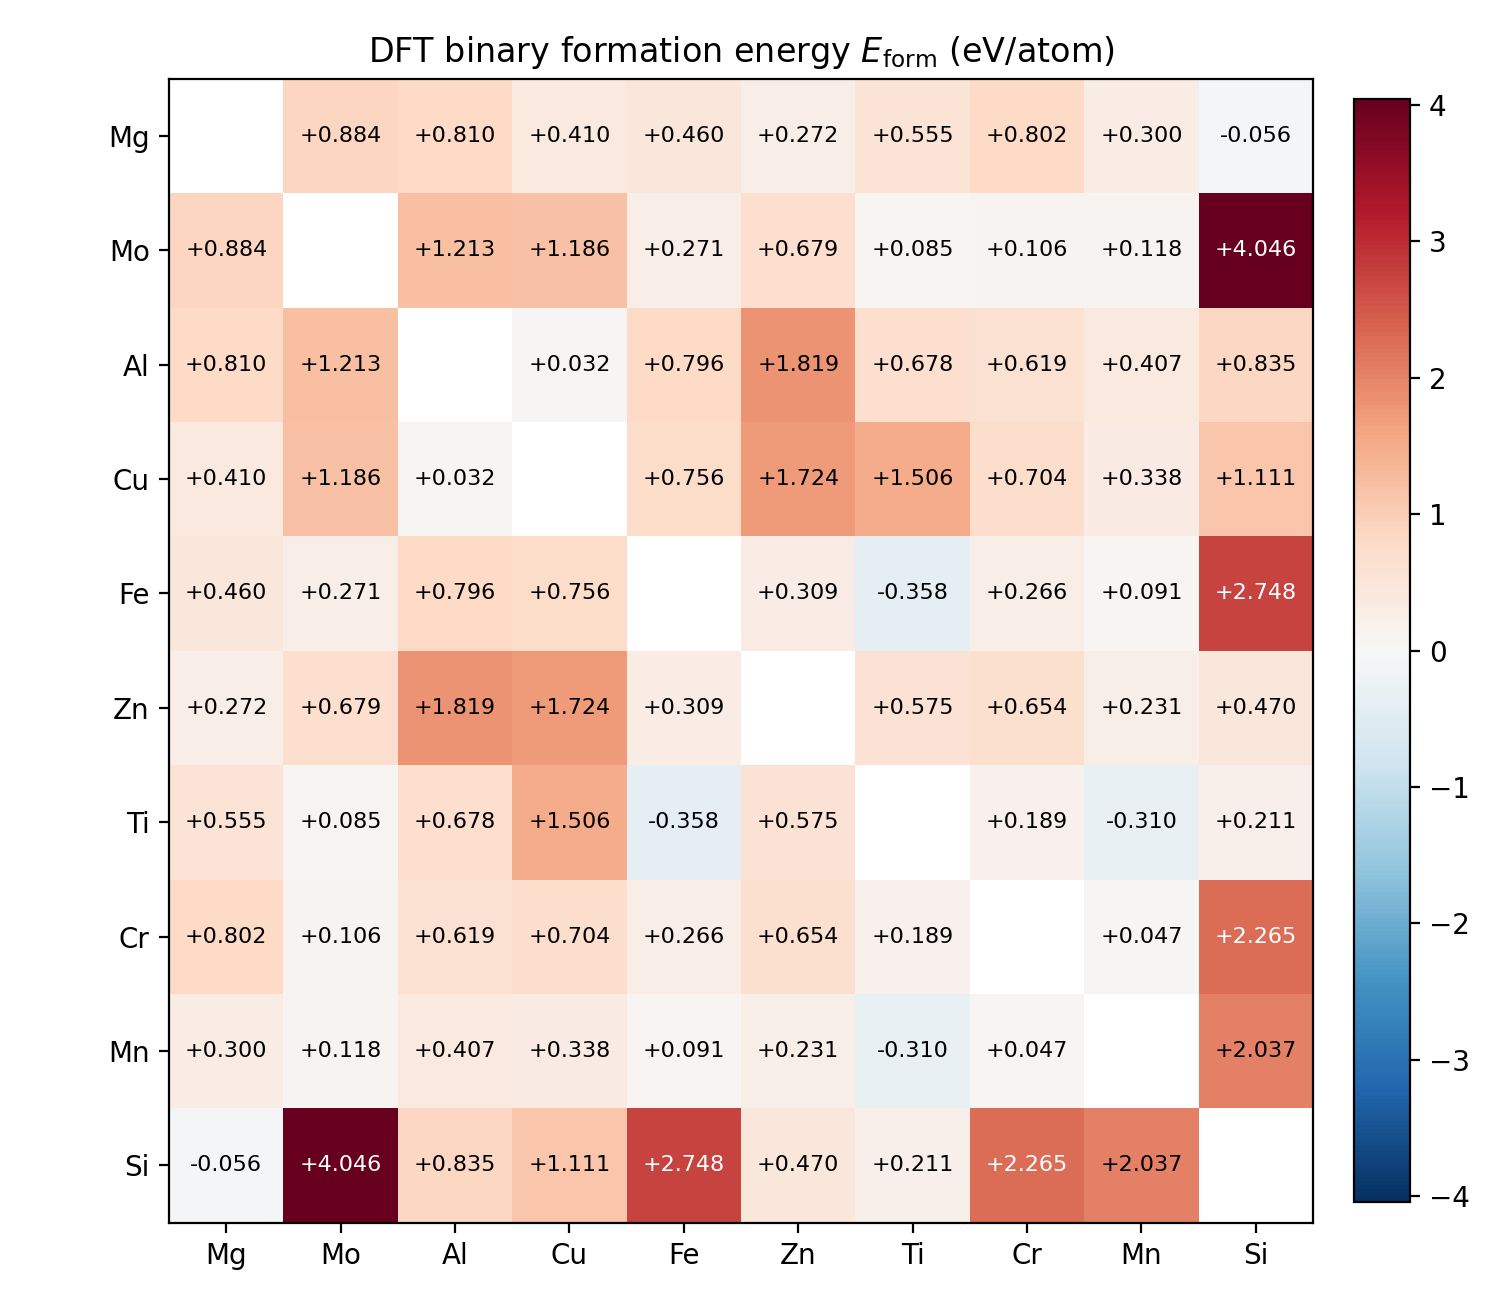
\includegraphics[height=3.7cm,keepaspectratio]{figures/formation_energy_heatmap.png}\\[-0.3em]
\scriptsize Binary formation energies $E_{\mathrm{form}}(i, j)$ (eV/atom):
negative $=$ exothermic mixing, positive $=$ limited solubility ---
these seed the MEAM cross-terms.

\smallskip
\begin{block}{Stage 4 --- single-element initialisation}
\scriptsize
Screening exponent from each DFT triple,\
$\alpha = a_{0}\sqrt{9 B \Omega / E_{\mathrm{coh}}}$
($\Omega$: cell volume)
$\to$ complete 12-element MEAM library ($\sim\!70$\,ms, cached).
$\alpha$-Mn EOS did not converge $\to$ relaxed-BCC approximation.
\end{block}
\end{columns}
\end{frame}
